\chapter{ExxonMobil Model}
\label{ch:exxonmobilmodel}

\section{Introduction}
The model is developed by Dixit and Manna in 2021, \referencename~\cite{ref:dixit2021a}. It is designed as a 2 DOF per node, axial-torsional system to model the dynamics of drill strings while drilling and tripping. Modeling is carried out as a lumped-parameter study. Also, the model incorporates bit-rock and friction models in order to investigate stick-slip effects. Governing equations are solved by a Runge-Kutta method using an ODE45 solver. 

\section{Model Description}
The model employs an axial-torsional system and uses a lumped-parameter technique.  The axial and torsional DOF are coupled through the friction terms.  There is not a coupling from material properties, the inertia terms, et cetera.  The model includes the ability to use different operational conditions and incorporation of heave compensator dynamics.  It allows for various components such as drill pipes, HWDP, drill collars, and mud-motors. Additionally, it integrates friction models to represent the axial and tangential forces acting along the drill string and includes a bit-rock interaction model (\referencename~\cite{ref:dixit2021a}). The governing equations of motion are solved by an ODE45 solver. Validation of the model was done by comparing simulation results with field data from rotational startups, off-bottom rotations, and post-connection operations. 

The equations of motion are coupled through friction terms. The model takes into account the velocity, well trajectory, and buoyancy effects when calculations of friction forces. Drag from drilling fluid is uniformly applied throughout the system. The friction model also has the following features:
\begin{bulletedlist}
    \item Friction model is coupled, the resultant velocity of the axial and torsional DOF are use to determine the friction force
    \item No movement until the resultant reaction force reaches static limit
    \item Coulomb friction model is implemented when the drill string is in motion \reviewcomment{How are both Coulomb and Stribeck friction used?}
    \item The friction state is tracked for each element
\end{bulletedlist}

The bit-rock interaction model is based on depth-of-cut and calculated by tracking the bit-depth relative to hole-depth. At each time step, the bit is considered to be drilling ahead when the DOC is higher than zero (the bit depth is greater than the hole depth) and the angular displacement of the bit is in the direction of the input rotation (i.e., the bit is not standing still or rotating backwards).  This feature contributes to a more realistic representation of the drilling process.

The Python-based source code is designed using a modular approach.  Most functions are distributed across separate Python files and are easily accessible by importing them. The code's operational instructions and guidelines are included in a manual (\referencename~\cite{ref:dixit2021a}), offering users guidance on running the code effectively.

\section{Top Drive Model}
The model utilizes the axial and rotational velocity of the top-drive as input. These are integrated to calculate the corresponding axial and rotational displacements of the top-drive.

Torque on top-drive can be derived as
\begin{equation}\label{TorqueEQ}
  \tau_{top\_drive} = k_{t1} \times \theta_{top\_drive}
\end{equation}
where $\tau_{top\_drive}$ is top-drive torque, $k_{t1}$ is torsional stiffness of first drill-string element, and $\theta_{top\_drive}$ is top-drive rotation angle. \reviewcomment{This equation and explanation still seems off.}

The model incorporates an additional parameter known as \emph{heave} which accounts for the influence of waves during offshore operations. If the current time surpasses the heave delay\reviewcomment{This needs clarification.}, additional computations are conducted to determine heave displacement and rate of penetration (ROP). These calculated values are subsequently added to the original top-drive ROP and displacement data. The heave ROP and displacement calculations are represented by the equations
\begin{equation}\label{Z_heave}
  Z_{heave} = x \cdot \sin(\omega \cdot (t - t_{heave\_delay}))
\end{equation}
\begin{equation}\label{ROP_heave}
  ROP_{heave} = x \cdot \omega \cdot \cos(\omega \cdot (t - t_{heave\_delay}))
\end{equation}
where 
$Z_{heave}$ and $ROP_{heave}$ are heave displacement and ROP, $x$ is heave amplitude, $\omega$ is heave angular velocity, $t$ is time and $t_{heave\_delay}$ is heave delay time.
 
\section{Bit Model}

The laws governing the bit-rock interface in drilling operations primarily rely on the relationships between weight on bit, torque on bit, rate of penetration, and angular velocity. These interdependent variables play a crucial role in achieving efficient drilling while also influencing the emergence of drilling dysfunctions within the system. The forces and torque exerted on the bit are directly influenced by the instantaneous changes in axial and angular velocities.

The interaction between PDC bits and the rock formation encompasses a combination of cutting and frictional contact, as identified by \referencename~\cite{ref:detournay1992a}.   This is modeled by decomposing the weight on bit and torque on bit into cutting and frictional components, which are contingent upon the strength of the rock formation being drilled.  The WOB and TOB are given as
\begin{equation}\label{WOB}
  WOB_{bit} = (k_{WOB}\times DOC_{iteration}) + (c_{bit-axial}\times \dot{Z}_{bit-ietration})
\end{equation}
\begin{equation}\label{Torque}
  TQ_{bit} = k_{TQ}\times DOC_{iteration\; array}\times (\pm1)
\end{equation}
where $k_{WOB}$ is the weight on bit coefficent, $k_{TQ}$ is the torque on bit coefficient, $DOC_{iteration}$ is depth of cut at the current time step, $C_{bit-axial}$ is axial viscous damping, and $Z$ is bit displacement.  The rock strength is incorporated into the coefficients $k_{WOB}$ and $k_{TQ}$.  The dependency on the depth of cut represents the material removed during drilling.

\section{Friction Model}
\sout{
Modeling friction forces along the drill string is a challenging task due to the system's nonlinear behavior, continuous changes in velocity, and a large combination of materials (formation, drilling fluid, et cetera). The net frictional force is highly influenced by the sliding velocity, with the axial component contributing to drag force and the tangential component generating torque within the system.}
\begin{figure}
	\begin{minipage}[t]{\linewidth}
			\begin{minipage}[t]{0.3\linewidth}
				\centering
				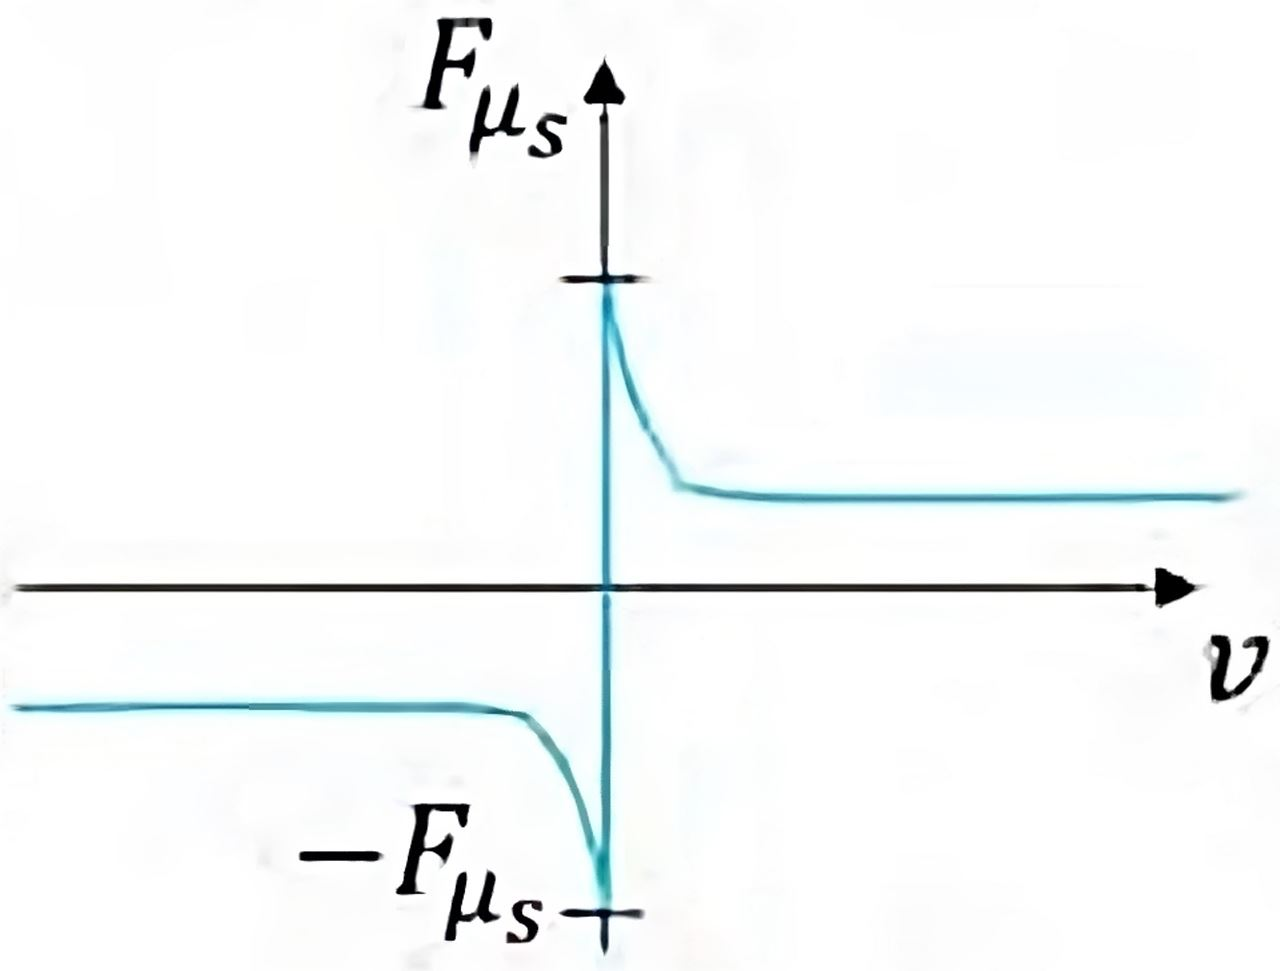
\includegraphics[width=0.90\linewidth]{stribeckfriction}
				\subcaption{Stribeck friction without fluid drag (\referencename~\cite{ref:cayeux2020a}).}
				\label{fig:stribeckfriction}
			\end{minipage}
			\hfill
			\begin{minipage}[t]{0.65\linewidth}
				\centering
				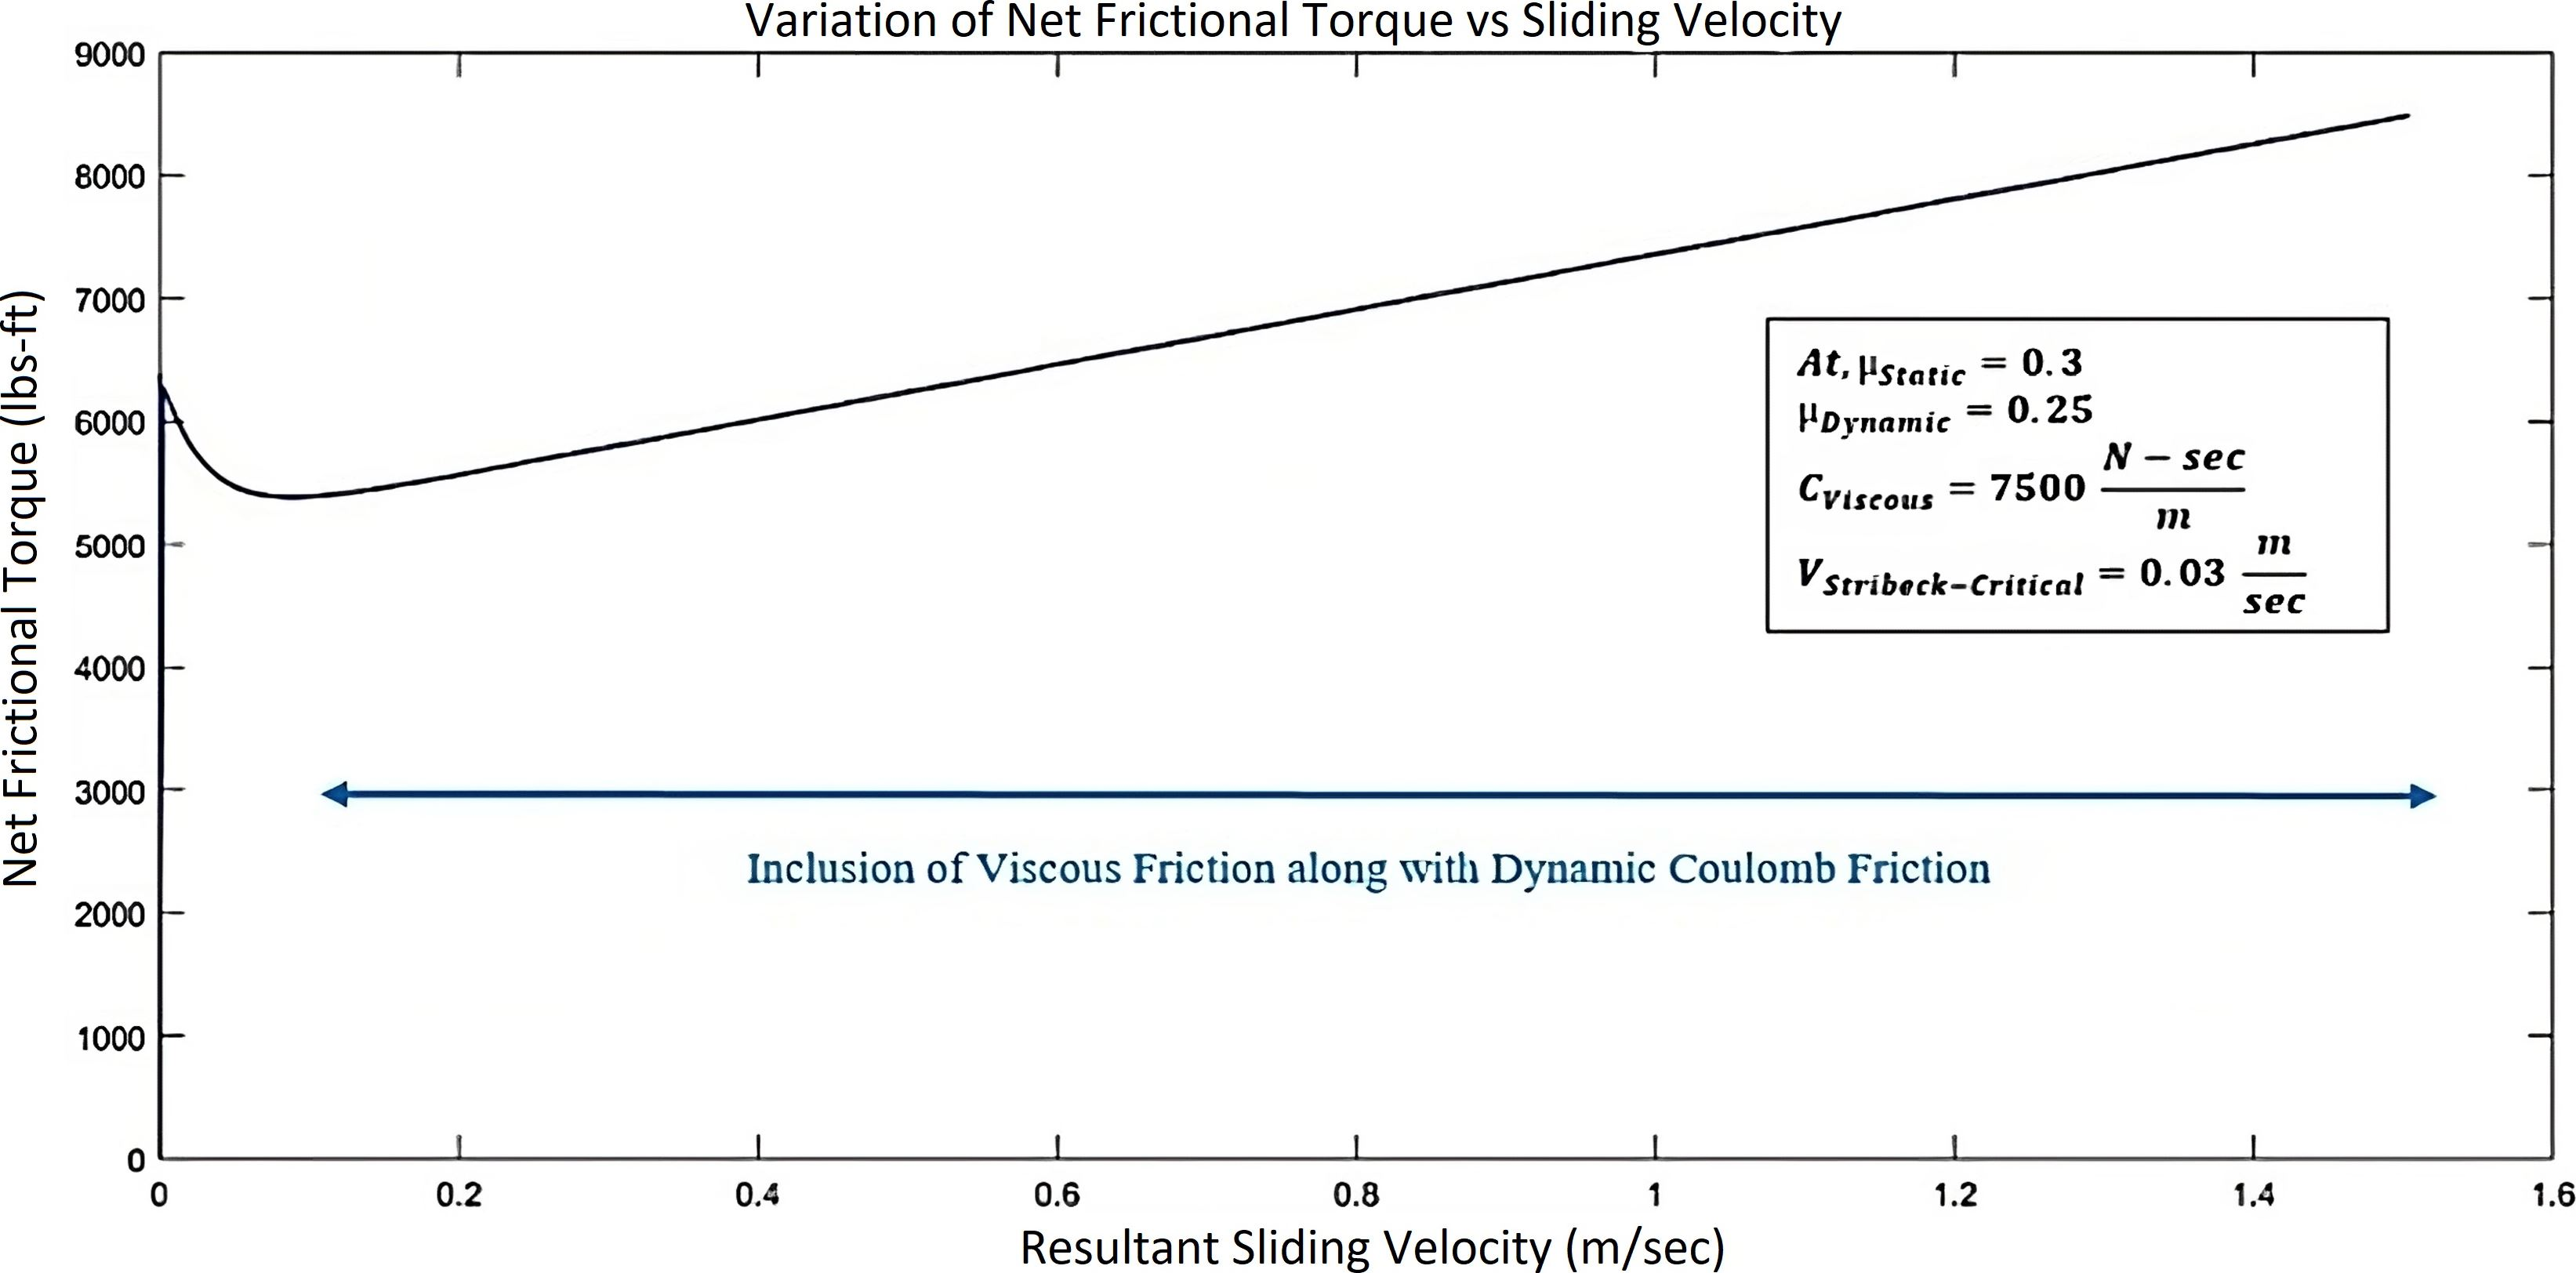
\includegraphics[width=\linewidth]{exxonmobilfriction}
				\subcaption{Stribeck friction with fluid drag as it used in the ExxonMobil model (\referencename~\cite{ref:dixit2021a}).}
				\label{fig:exxonmobilfriction}
			\end{minipage}
	\end{minipage}
	\caption[Comparison of friction models]{A comparison of Stribeck friction without fluid drag in~(\subref{fig:stribeckfriction}) and the Stribeck friction with fluid drag that is used in the ExxonMobil software in~(\subref{fig:exxonmobilfriction}).}\label{fig:frictionmodels}
\end{figure}
%\begin{figure}[!hbt]
%  \centering
%  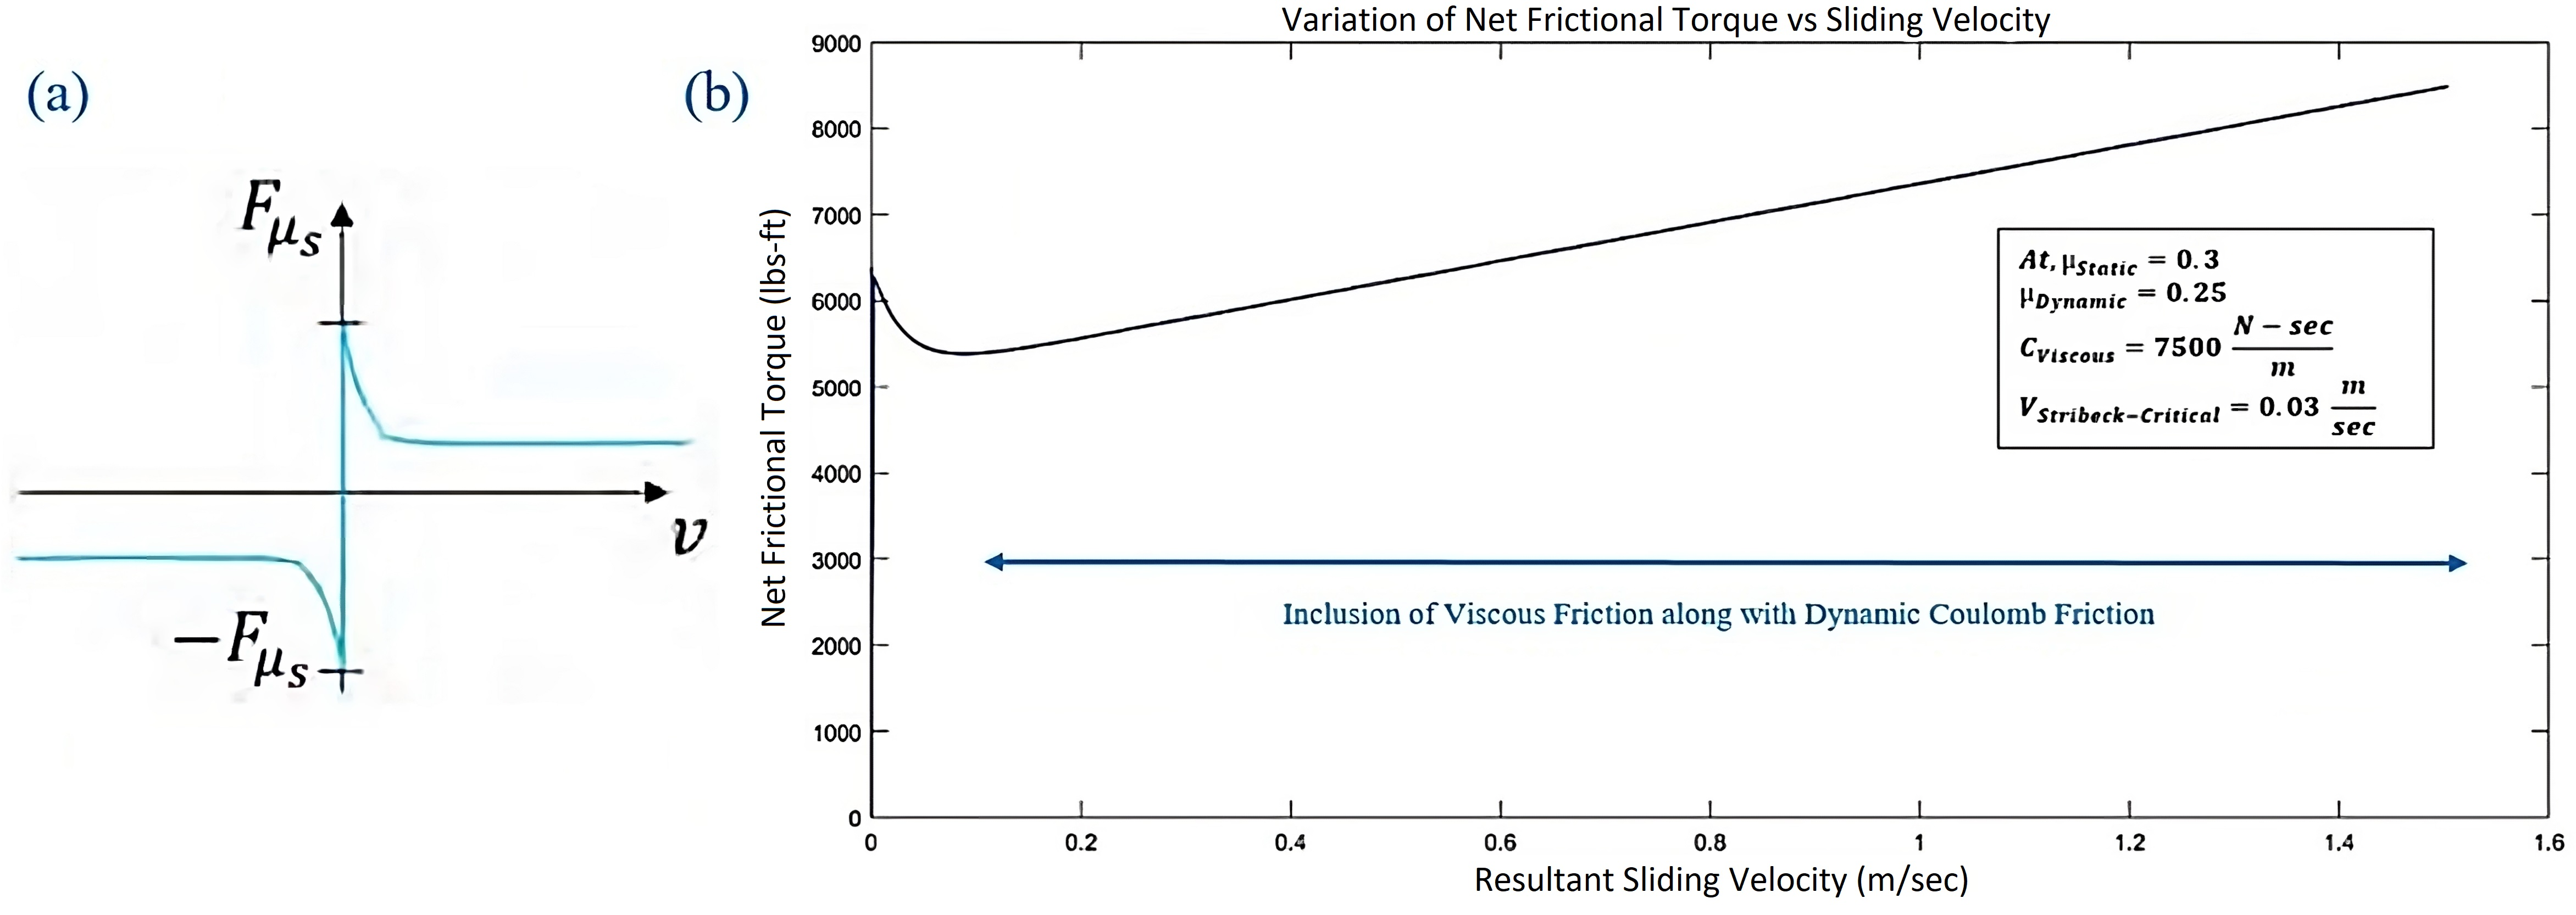
\includegraphics[width=\linewidth]{Stribeck}
%  \caption[Comparison of friction models]{Friction models: a) without fluid drag (\referencename~\cite{ref:cayeux2020a}), b) Coulomb + fluid drag (\referencename~\cite{ref:dixit2021a})}\label{Friction models}
%\end{figure}

\sout{
To enhance the assessment of frictional forces at the bit and along the length of the drill string, particularly in deviated wellbores, a friction model (\referencename~\cite{ref:cayeux2020a}) is implemented within the drilling simulator.}
\sout{
As the force of friction increases, it introduces a negative damping effect}\needsclarification[How so?]\sout{as the sliding velocity approaches zero. This negative damping effect can lead to stick-slip dysfunction, even when the bit is not in contact with the bottom of the well. The axial and rotational displacement and velocity of the top drive do not instantaneously transfer to the bit. The elements of the drill string must overcome inertia and static friction to transfer energy to the next element. This lag in energy transfer can be effectively described by the Stribeck curve, where the frictional forces decrease as the velocity increases (see } \figurename~\ref{fig:frictionmodels}).
\sout{
The Stribeck friction has the negatively sloped characteristics taking place at low velocities (see \figurename~\ref{fig:stribeckfriction}). The Coulomb friction results in a constant force at any velocities. The fluid drag}\footnote{It is called ``viscous friction`` in the manual.}\sout{ opposes motion with the force directly proportional to the relative velocity which is shown in \figurename~\ref{fig:exxonmobilfriction}. The sum of the Coulomb and Stribeck frictions at the vicinity of zero velocity is often referred to as the breakaway friction.}
%\footnotetext{It is called ``viscous friction'' in the manual.}
\begin{equation}\label{dynamic_force}
  F_{\mu,k} = \mu_{k}\times F_{n} \times (-V_{Sliding})
\end{equation}
\sout{
where $F_{\mu,k}$ is dynamic friction force, $\mu_k$ is dynamic friction factor, $F_n$ is the normal force, and $V_{sliding}$ is sliding velocity.
The static friction force opposes the direction of axial motion (\equationname~\ref{dynamic_force}), while static friction force $F_{\mu,s}$ acts in the opposite direction of the sum of all tangential forces when there is no sliding motion $V_{Sliding}=0$.}\reviewcomment{Why would dynamic be only in the axial direction?  Why is static the sum only when there is not motion?  \sout{This seems like it was rushed in the original document and needs to be checked.}The magnitude of the static friction force is equal to the sum of all tangential forces. That is, the condition}
\begin{equation}\label{zero}
  F_{\mu,s} + \sum F_{Ext} = 0
\end{equation}
\sout{
where $F_{\mu,s}$ is static friction force and $\sum F_{Ext}$ is the sum of external forces, is valid when there is no sliding motion $V_{Sliding}=0$.
If dynamic friction force calculated above is less than $\mu_{s}\times F_{n}$, where $\mu_{s} > \mu_{k}$, then the surface is not sliding.}

The mechanical friction is modeled as Coulomb friction based on Stribeck effect. The static friction applies when there is no slip ($\vec{v}_s$=0), where the velocity vector, $\vec{v}_s$, is a function of rotational and axial velocities of the pipe. More details for the velocity vector can be seen from [Cayeux. 2018]. The magnitude and direction of the static friction force are equal and opposite to that of the external force at contact point, respectively (\equationname~\ref{eq:exxon_staticFF}). On the other hand, dynamic friction applies when the pipe starts to slide ($\vec{v} > 0$). The dynamic friction acts in the opposite direction to the velocity vector. The equation of dynamic friction force is shown in \equationname~\ref{eq:exxon_dynamicFF}, where $\mu_k$ is kinetic friction factor and $\vec{F_n}$ is the normal force at the drill string.

\begin{equation}\label{eq:exxon_staticFF}
  F_{\mu,s} + \sum F_{Ext} = 0
\end{equation}

\begin{equation}\label{eq:exxon_dynamicFF}
  \vec{F_{\mu k}} = -\mu_k ||{\vec{F_n}}||\frac{\vec{v}_s}{{||\vec{v}_s}||}
\end{equation}


In order to avoid the discontinuities when $V_s$ tends to zero, a Stribeck friction model is used. The following \equationname~\ref{Stribeck velocity} was proposed by (\referencename~\cite{ref:tustin1947a})
\begin{equation}\label{Stribeck velocity}
F_{\mu} = F_{\mu,k} + (F_{\mu,ks} - F_{\mu,k})\times e^{-\frac{|V_s|}{V_{CS}}}
\end{equation}
where $F_{\mu}$ is friction applied in the drill string and $V_{CS}$ is Stribeck critical velocity. \figurename~\ref{fig:stribeckfriction} illustrates the Striebec friction force as a function of sliding velocity. However, It should be noted that the model does not account for capstan effects.\reviewcomment{DY: what is capstan effect? do we have to leave this?} 

Furthermore, the order of the viscous damping constants is maintained consistently to ensure that the system remains in an ideal damp state, aligning with the field data. Values of viscous dampers are held constants during simulation, but the viscous frictional force will vary depending on the sliding velocities as can be seen in \figurename~\ref{fig:exxonmobilfriction}. 

Below, the friction model input parameters are listed. \reviewcomment{DY: maybe we can remove this?}
\begin{bulletedlist}
    \item Equivalent diameter of pipe
    \item Coulomb friction force
    \item Coulomb friction force axial component
    \item Coulomb friction force tangential component
    \item Coulomb friction torque tangential component
    \item Viscous friction force axial component
    \item Viscous friction force tangential direction component
    \item Axial and tangential components of net frictional force and torque
\end{bulletedlist}

\section{Mathematical Background}

The set of partial differential equations that describe the motion of the drill-string can be combined into a coupled axial-torsional system of second-order differential equations. 

\begin{align}\label{Governing equations}
     m_{i}\dfrac{\partial^{2}s_{i}}{\partial t^{2}} & = -k_{a,i}(s_{i}-s_{i-1}-l_{i}) + k_{a,j+1}(s_{i+1}-s_{i}-l_{i+1}) + \sum{F_{ext, i}} \\
     I_{i}l_{i}\dfrac{\partial^{2}\theta_{i}}{\partial t^{2}} & = -k_{t,i}(\theta_{i}-\theta_{i-1}-l_{i}) + k_{t,j+1}(\theta_{i}-\theta_{i+1}) + \sum{\tau_{ext,/ i}}
\end{align}

To convert these equation sets into vector form, we can represent the variables and their derivatives as vectors.

\begin{align}
  \{M\} \ddot{\boldsymbol{Z}}+\left\{C_a\right\} \dot{\boldsymbol{Z}}+\left\{K_a\right\} \boldsymbol{Z}+\boldsymbol{f}_{\text {fric }} &= \boldsymbol{F}_{\text {forcing }} \label{eq:em_axial_vector_form}\\
  \{J\} \ddot{\boldsymbol{\theta}}+\left\{C_t\right\} \dot{\boldsymbol{\theta}}+\left\{K_t\right\} \boldsymbol{\theta}+\boldsymbol{\tau}_{\text {fric }} &= \boldsymbol{\tau}_{\text {forcing }} \label{eq:em_torsional_vector_form}
\end{align}


\begin{align}
	\{M\} &= \left[\begin{array}{ccc}
				m_1 & \cdots & \vdots \\
				\vdots & \ddots & \vdots \\
				\vdots & \cdots & m_n
				\end{array}\right] \\
	\{J\} &= \left[\begin{array}{ccc}
			J_1 & \cdots & \vdots \\
			\vdots & \ddots & \vdots \\
			\vdots & \cdots & J_n  \\
  			\end{array}\right] \\
	\left\{C_a\right\} &= \left[\begin{array}{ccc}
							c_{a 1} & \cdots & \vdots \\
							\vdots & \ddots & \vdots \\
							\vdots & \cdots & c_{a n}
							\end{array}\right] \\
	\left\{C_t\right\} &= \left[\begin{array}{ccc}
							c_{t 1} & \cdots & \vdots \\
							\vdots & \ddots & \vdots \\
							\vdots & \cdots & c_{t n}
							\end{array}\right] \\
 	\left\{K_a\right\} &= \left[\begin{array}{ccc}
							k_{a 1} & -k_{a 2} & \cdots \\
							-k_{a 2} & \ddots & \vdots \\
							\vdots & \cdots & k_{a(n-1)}+k_{a n}
							\end{array}\right] \\
	\left\{K_t\right\} &= \left[\begin{array}{ccc}
							k_{t 1} & -k_{t 1} & \cdots \\
							-k_{t 1} & \ddots & \vdots \\
							\vdots & \cdots & k_{t(n-1)}+k_{t n}
							\end{array}\right] \\
  	F_{\text {forcing }} &= \left[\begin{array}{c}
							\boldsymbol{k}_{a 1} \cdot Z_{\text {top\_drive}} \\
							\vdots \\
							-\boldsymbol{k}_{a\_\text{bit}} \cdot \text {DOC}
							\end{array}\right] \\
	\mathcal{T}_{\text {forcing }} &= \left[\begin{array}{c}
							\boldsymbol{k}_{t 1} \cdot \theta_{\text {top\_drive}} \\
							\vdots \\
							-\boldsymbol{k}_{t\_\text{bit}} \cdot \text {DOC}
							\end{array}\right]
	\label{eq:emmatrixform}
\end{align}


\begin{mathwhere}[1.0in]
\mathdefitem{Z_0}{$\int V_0\ dt$}
\mathdefitem{m_n}{drill string element mass}
\mathdefitem{Z}{position (downward direction considered as positive)}
\mathdefitem{k_a}{axial stiffness of drill-string element}
\mathdefitem{V_o}{Top-drive (draw-works) axial velocity as input}
\mathdefitem{Z_{top\_drive}}{Top-drive (draw-works) axial displacement as input}
\mathdefitem{\dot{Z}}{bit axial velocity (downward direction considered as positive)}
\mathdefitem{WOB_{Surface}}{Surface/Top-drive WOB (In ROP Control Mode)}
\mathdefitem{J_n}{mass moment of inertia of drill string element}
\mathdefitem{\theta}{rotation angle (Clockwise direction is considered as positive)}
\mathdefitem{\omega_o}{top drive angular velocity as input}
\mathdefitem{\theta_{top\_drive}}{top drive rotation as input}
\mathdefitem{k_t}{Torsional stiffness of drill-string}
\mathdefitem{\dot{\theta}}{bit rotary velocity (Clockwise direction considered as positive)}
\mathdefitem{TQ_{Surface}}{Surface/Top-drive Torque}
\end{mathwhere}

The differential equation sets are solved using the ODE45 solver.\ This solver is chosen for its efficiency in computational calculations.


\section{Findings and Code Modifications}
 
One of the features of this model is simulation of ``on-bottom`` case for drilling. \figurename~\ref{findings} illustrates the typical output for that specific case.

During testing, we encountered an issue with the ``on-bottom'' case, specifically related to the bit-rock interaction model. The code was not displaying the ``drilling'' mode, indicating a constant value of depth of cut (DOC) and bit depth. Upon thorough investigation, we identified the root cause as the improper assignment of bit depth to bit displacement. Implementing a slight modification, the original bit depth was incorporated into the bit displacement calculation, thus accurately representing the actual bit depth during drilling. This change, along with other adjustments, successfully activated the ``drilling'' mode, enabling dynamic changes in both hole depth and non-zero DOC. More analysis can be found in \appendixname~\ref{ch:appendixexxonmobil}. 

\begin{figure}
  \centering
  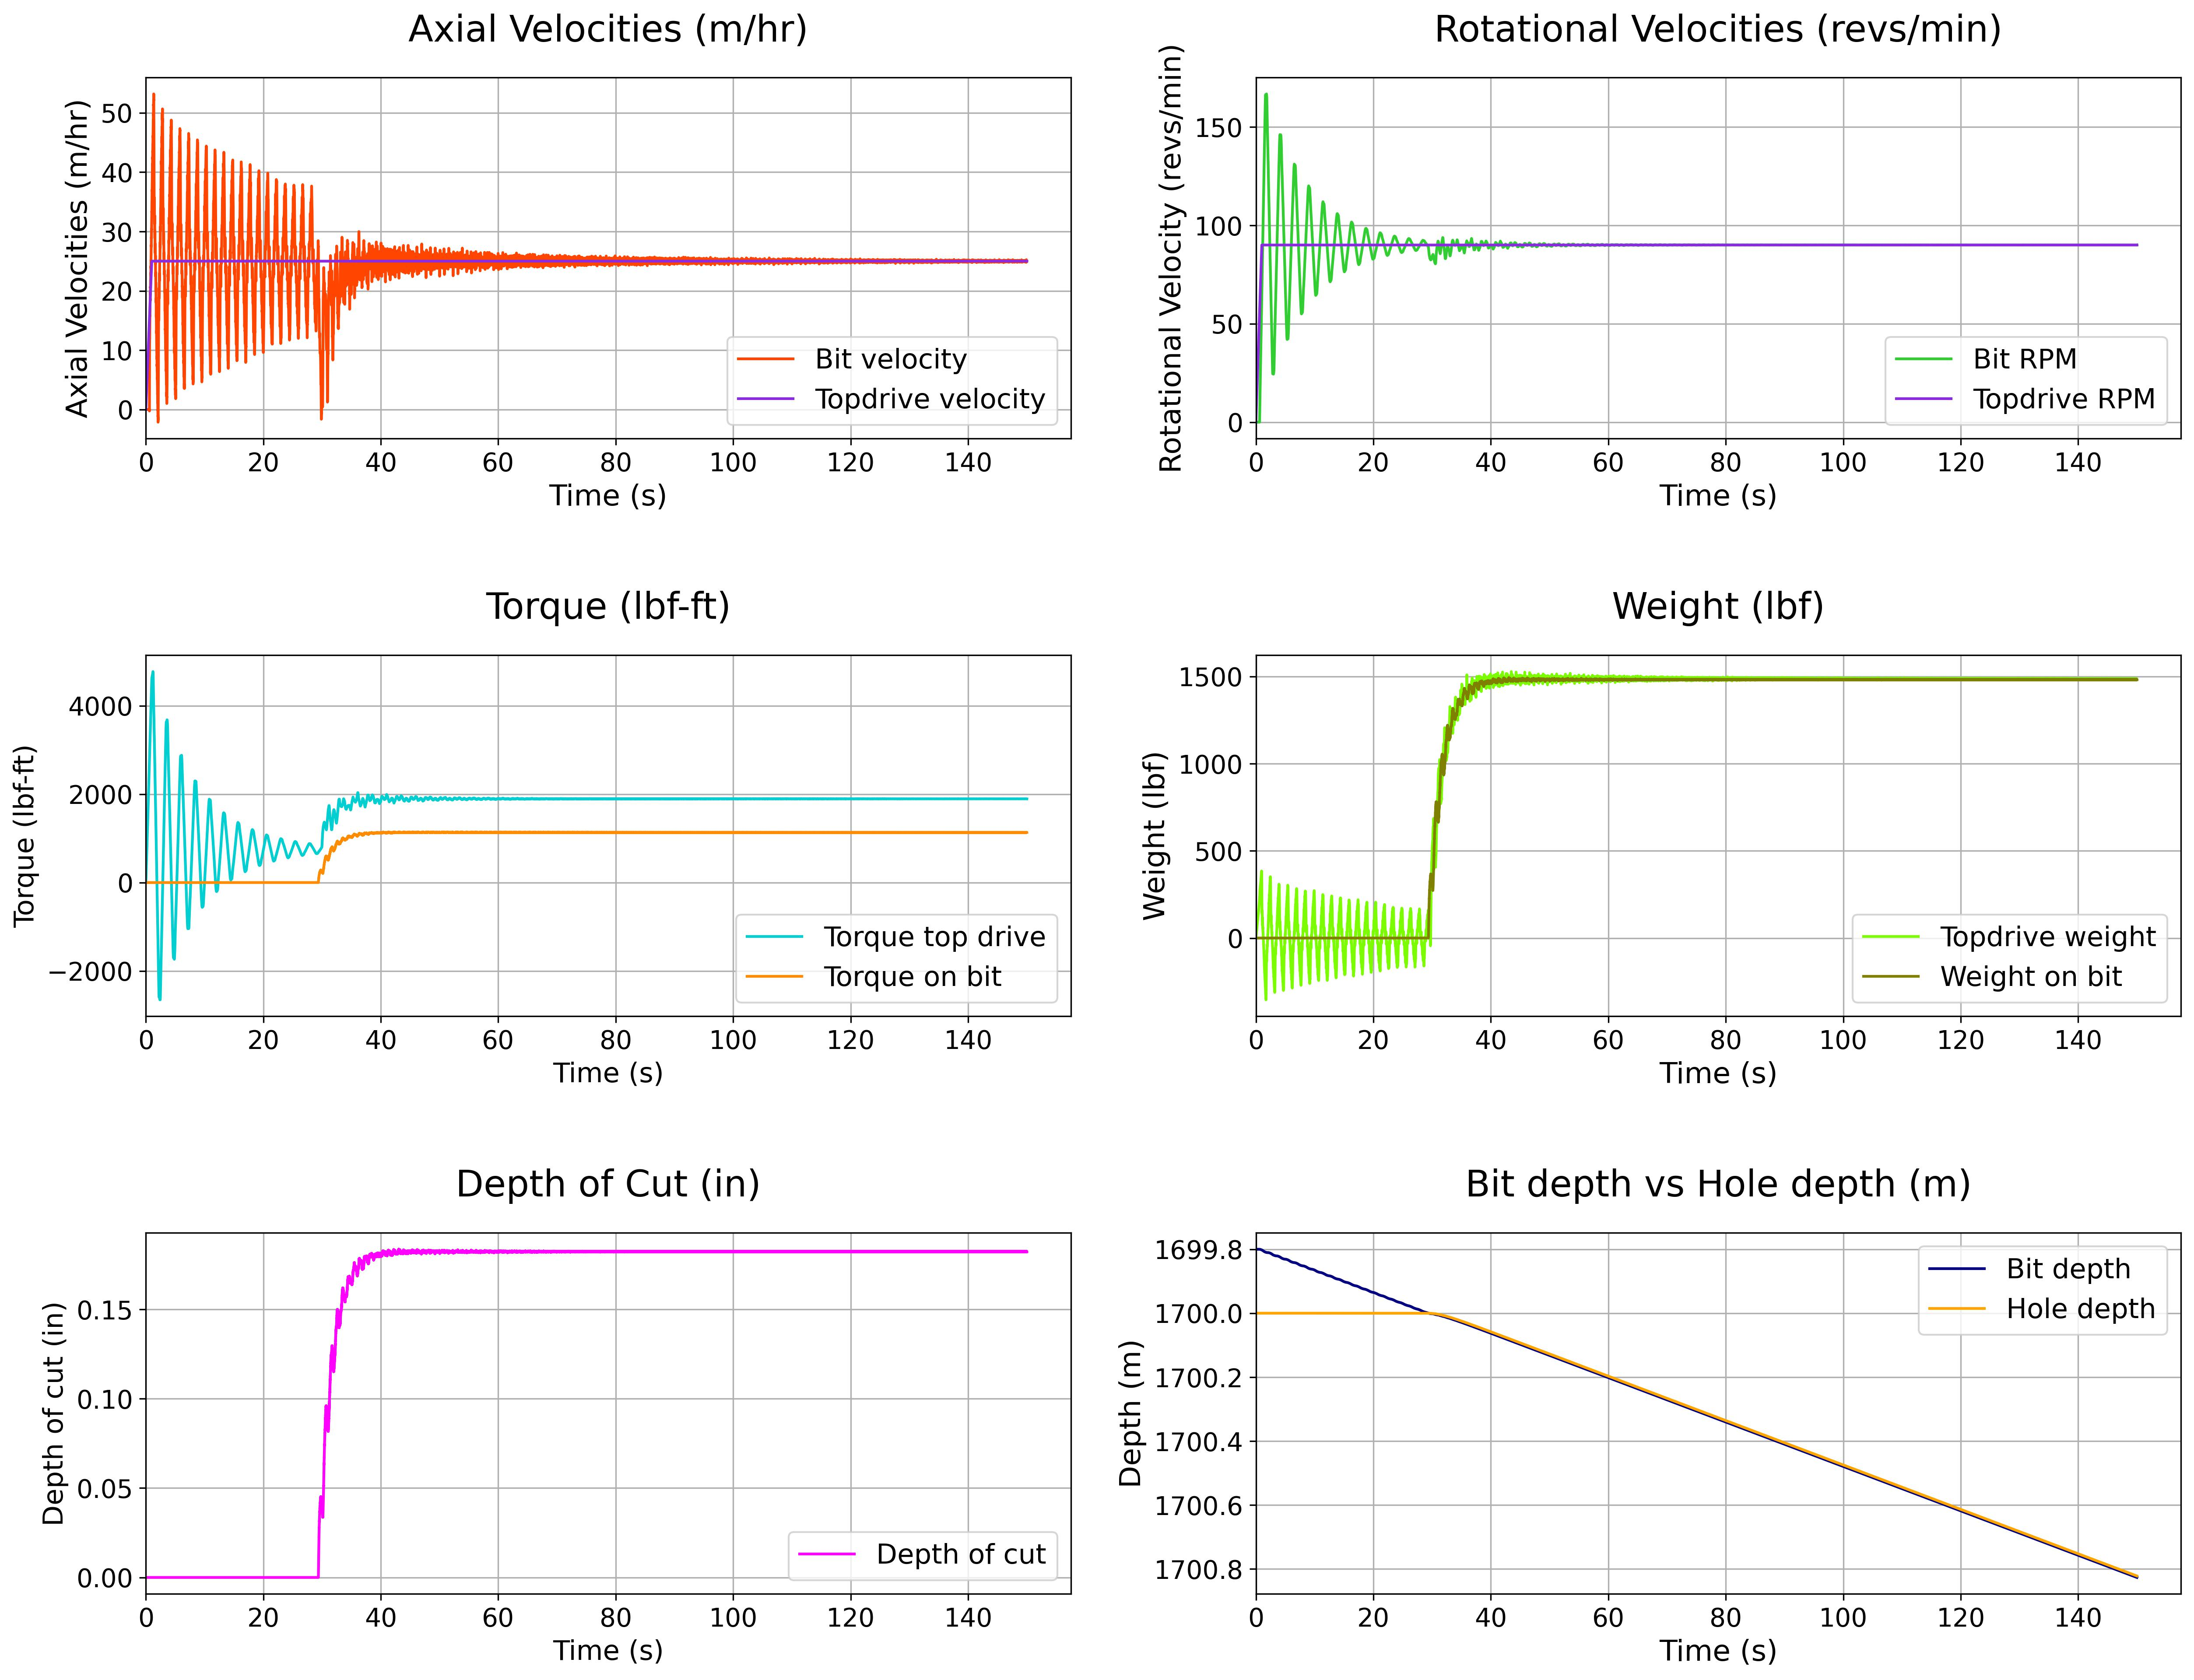
\includegraphics[width=\linewidth]{on_bottom}
  \caption[Plots of on-bottom case]{Plot of drilling parameters for on-bottom case.}\label{findings}
\end{figure}

